\documentclass{article}
\usepackage{graphicx}
\usepackage{paralist} % needed for compact lists
\usepackage[normalem]{ulem} % needed by strike
\usepackage[urlcolor=blue,colorlinks=true]{hyperref}

\title{HPC}
\author{JCN-9000}
\begin{document}
\date{2019-05-10}
\maketitle
\clearpage


\section*{Definition}

\begin{description}
\item[\htmladdnormallink{HPC}{https://tinyurl.com/yycxbun4}]

    HPC systems tend to focus on tightly coupled parallel jobs, and as
    such they must execute within a particular site with low-latency
    interconnects.

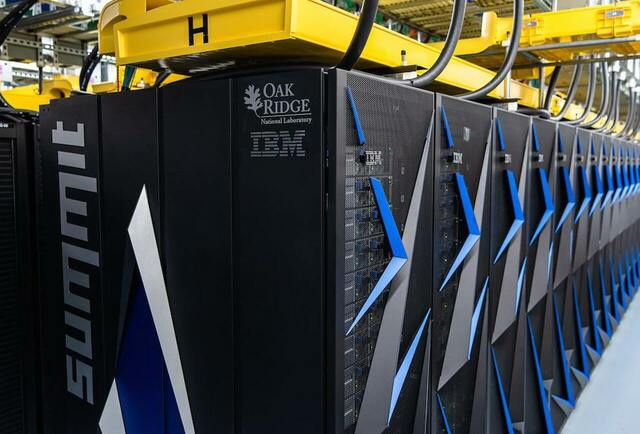
\includegraphics{images/Summit_small.jpg}
\end{description}

\section*{Wikipedia IT}

\begin{description}
\item[\htmladdnormallink{HPC}{https://tinyurl.com/yycxbun4IT}]

    Con High Performance Computing (HPC) (in italiano calcolo ad
    elevate prestazioni), in informatica, ci si riferisce alle
    tecnologie utilizzate da computer cluster per creare dei sistemi di
    elaborazione in grado di fornire delle prestazioni molto elevate
    nell'ordine dei PetaFLOPS, ricorrendo tipicamente al calcolo
    parallelo.
\end{description}

\section*{TOP 500}

\begin{compactitem}
\item \htmladdnormallink{TOP$\backslash$_500}{https://www.top500.org/}
\item \htmladdnormallink{LIST}{https://www.top500.org/lists/2018/11/}
\item \htmladdnormallink{1-100}{https://www.top500.org/list/2018/11/?page=1}
\end{compactitem}

\section*{IPC - Process}

\begin{compactitem}
\item shared files / memory + semaphores
\item \htmladdnormallink{pipes (named, unnamed)}{https://opensource.com/article/19/4/interprocess-communication-linux-channels}
\item message queues                unidirectional
\item sockets (memory, network )    bi-directional
\item signals
\item \htmladdnormallink{RPC}{https://en.wikipedia.org/wiki/Remote$\backslash$_procedure$\backslash$_call}
  \begin{compactitem}
  \item ONC/RPC, XML-RPC -$>$ SOAP, CORBA, JSON-RPC, gRPC, ...
  \end{compactitem}
\end{compactitem}

\section*{Approaches to message passing}

\begin{compactdesc}
\item[PVM]
    Parallel Virtual Machine
    \htmladdnormallink{PVM}{https://en.wikipedia.org/wiki/Parallel$\backslash$_Virtual$\backslash$_Machine}
\item[MPI the Message Passing Interface]
    \htmladdnormallink{MPI}{https://tinyurl.com/6mfo5pf}
\end{compactdesc}

\section*{MPI}

--map-by hwthread
--rank-by hwthread
--bind-to hwthread
--use-hwthread-cpus

mpirun --use-hwthread-cpus --bind-to hwthread -np 4

mpirun --map-by node    : balanced - rrobin
mpirun -nolocal

mpirun --use-hwthread-cpus --bind-to hwthread -np 1 search$\backslash$_mpi
  Elapsed wallclock time is 59.731
mpirun --use-hwthread-cpus --bind-to hwthread -np 2 search$\backslash$_mpi
  Elapsed wallclock time is 44.0702
mpirun --use-hwthread-cpus --bind-to hwthread -np 3 search$\backslash$_mpi
  Elapsed wallclock time is 31.4417

\section*{Pelican HPC}

\htmladdnormallink{https://www.pelicanhpc.org/index.html}{https://www.pelicanhpc.org/index.html}

\section*{PelicanHPC over Virtualbox}

First Steps ...
sudo mkdir /cdrom
sudo mount -oro /dev/sr1 /cdrom
sudo /cdrom/VBoxLinuxAdditions.run

sudo ln -sf /home/etc/apt/sources.list /etc/apt/sources.list
sudo apt update
sudo apt install libatlas3-base
sudo apt install gpm

cd hpl-2.0
sh SetupForPelican
cd bin/Pelican HPC
orterun --hostfile /home/usr/tmp/bhosts -np 4 xhpl

\section*{PelicanHPC over KVM}

\section*{URLS}

\htmladdnormallink{HPC}{https://www.techopedia.com/definition/4595/high-performance-computing-hpc}

FLOPS Unit Peta Exa  \htmladdnormallink{https://en.m.wikipedia.org/wiki/Unit$\backslash$_prefix}{https://en.m.wikipedia.org/wiki/Unit$\backslash$_prefix}
Q commands
Queuing system
Hardware components
Power Supply
CPU
GPU
Network
Infiniband
Intel OmniPath
Fast Ethernet
Shared Filesystem
NFS
Lustre Gluster BeeGFS
MP. Hibrid: threads + process
OpenMPI - OpenMP
PlatformMPI
IntelMPI
\htmladdnormallink{https://github.com/wiki2beamer/wiki2beamer}{https://github.com/wiki2beamer/wiki2beamer}
\htmladdnormallink{https://openhpc.community}{https://openhpc.community}

\clearpage

EOD

\clearpage

/home/avaresio/GIT/txt2tags/txt2tags -t aapp --slides Slides.t2t
enscript -l -r -p file.ps Slides.aapp
ps2pdf file.ps Slides.pdf

pandoc -s -t beamer -o Slides.tex Slides.t2t
pdflatex Slides.tex $>$ Slides.pdf

impressive -f -g 1024x768 Slides.pdf

% LaTeX2e code generated by txt2tags 2.6. (http://txt2tags.org)
% cmdline: txt2tags -t tex Slides.t2t
\end{document}
